\chapter{Background}

\section{Markov Decision Process}

Markov Decision Processes (MDPs) are a classical formalization of sequential decision making under uncertainty, where actions influence not just immediate responses, but also subsequent situations. Hence an MDP can be described as a controlled \textit{Markov chain}\footnote{A sequence of random variables $X_0, X_1, . . . $ with values in a countable set $S$ is a \textit{Markov chain} if at any time $n$, the future states (or values) $X\textsubscript{n+1}, X\textsubscript{n+2}, . . .$ depend on the history $X_0, . . . , X_n$ only through the present state $X_n$ \cite{konstantopoulos2009markov}.}, where the control is given at each step by the chosen action. In this chapter the structure of an MDP and many techniques to solve its, are presented.

\subsection{Definition} Markov decision processes are defined as controlled stochastic processes satisfying the \textit{Markov property}\footnote{A stochastic process has the \textit{Markov property} if the probabilistic behaviour of the chain in the future depends only on its present value and discards its past behaviour.} and assigning reward values to state transitions~\cite{Put94}.  Formally, they are described by the $5$-tuple ($S$, $A$, $T$, $p()$, $R()$) where:

\begin{itemize}
	\item $S$ is the state space in which the process’ evolution takes place;
	\item $A$ is the set of all possible actions which control the state dynamics;
	\item $T$ is the set of time steps where decisions need to be made;
	\item $p()$ denotes the state transition probability function;
	\item $R()$ provides the reward function defined on state transitions.	
\end{itemize}

\paragraph{States} The set of environmental states $S$ is defined as the finite set $\{s_1, . . . , s_N\}$ where the size of the state space is $N$, i.e. $|S| = N$~\cite{wiering2012reinforcement}. Each state ${s \in S}$ is a vector of attributes (\textit{state variables}) that describes the current configuration of the system~\cite{Nevmyvaka}. More specifically, a state variable is the minimally dimensioned function of history that is necessary and sufficient to compute the \textit{state of knowledge}~\cite{Powell}.

\paragraph{Actions} The set of actions $A$ is defined as the finite set $\{a_1, . . . ,a_K\}$ where the size of the action space is $K$, i.e. $|A| = K$. Actions can be used to control the system state. The set of actions that can be applied in some particular state $s \in S$, is denoted $A(s)$, where $A(s) \subseteq A$. In more structured representations the fact that some actions are not applicable in some states, is modelled by a precondition function : $S$ × $A→{true,false}$, stating whether action $a \in A$ is applicable in state $s \in S$~\cite{wiering2012reinforcement}.

\paragraph{Time Steps} The set of time steps $T$ is defined as the finite set $\{t_1, . . . ,t_M\}$ where the size of the action space is $M$, i.e. $|T| = M$. Speaking about time a distinction between \textit{epochs} and \textit{episodes} has to be made. An episode consists of a fixed number of epochs. An epoch is the smallest time unit in an MDP.

\paragraph{Transition Probability} The transition probabilities $p()$ characterize the state dynamics of the system, i.e. indicate which states are likely to appear after the current state. For a given action $a$, $p(s'|s,a)$ represents the probability for the system to transit to state $s'$ after undertaking action $a$ in state $s$. This $p()$ function is usually represented in a matrix form where $P_a$ is the $|S|$ x $|S|$ matrix containing elements $\forall s, s', P\textsubscript{a, s, s'} = p(s'|s,a)$. Since each line of these matrices sums to one, the $P_a$ is said to be stochastic. The $p()$ probability distributions over the next state $s'$ follow the fundamental property which gives their name to Markov Decision Processes. If one writes $h_t = (s_0, a_0, ..., s\textsubscript{t-1}, a\textsubscript{a-1}, s_t)$ (the history of states and actions until time step $t$), then the probability of reaching state $s\textsubscript{t+1}$ consecutively to action $a_t$ is only a function of $a_t$ and $s_t$, and not of the entire history $h_t$~\cite{Sigaud:2010:MDP:1841781}. This concept can be easily resumed through the following equation :

\begin{equation}
	\forall h_t, a_t, s\textsubscript{t+1} \quad P(s\textsubscript{t+1} | h_t, a_t) = P(s\textsubscript{t+1} | s_t, a_t) = p(s\textsubscript{t+1} | s_t, a_t)
\end{equation}

\paragraph{Reward Function} The reward function specifies rewards for being in a state, or doing some action in a state. The state reward function is defined as $R : S \rightarrow \mathbb{R}$, and it specifies the reward obtained in states. The reward function is an important part of the MDP that specifies implicitly the \textit{goal} of learning. Thus, the reward function is used to give direction in which way the system, i.e. the MDP, should be controlled~\cite{wiering2012reinforcement}. It is critical that the reward set up truly indicate the goal that has to be accomplished. If the achievement of sub-goals is rewarded, then the agent might find a way to achieve them without achieving the real, final goal. Reward signal is the way of communicating the agent \textit{what} goal to achieve, not \textit{how} the goal has to be achieved~\cite{SuttonBarto}.

\begin{figure}[h!]
	\centering
	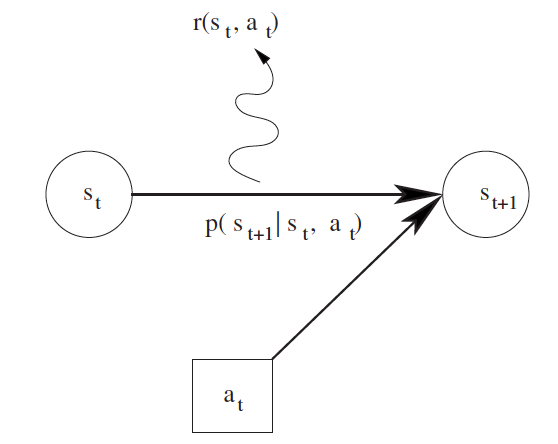
\includegraphics[width= 8cm, height = 7cm]{MDP.png}
	\caption{Markov decision process~\cite{Sigaud:2010:MDP:1841781}.}
	\label{fig:MDP}
\end{figure}

Markov decision processes allow to model the state evolution dynamics of a stochastic system when this system is controlled by an agent choosing and applying the actions $a_t$ at every time step $t$. The procedure of choosing such actions is called an action policy, or strategy, and is written as $\pi$~\cite{Sigaud:2010:MDP:1841781}.

\paragraph{Policy} Formally, given an MDP $\bigl\langle S, A, T, p(), R() \bigr\rangle$, a policy is a computable function that outputs, for each state $s \in S$, an action $a \in A(s)$~\cite{wiering2012reinforcement}. A policy can decide deterministically upon the action to apply or can define a probability distribution over the possible applicable actions. Then, a policy can be based on the whole history $h_t$ (history-dependent policy) or can only consider the current state $s_t$. Thus, four main families of policies can be defined (\ref{table:T1}).

\begin{table}[h!]
\centering
\begin{tabular}{|c|c|c|}
	\hline \textbf{Policy $\pi_t$}
	&\textbf{Deterministic} & \textbf{Stochastic}  \\ 
	\hline
	\hline Markov 
	&$s_t \rightarrow a_t$  &$a_t, s_t \rightarrow [0, 1]$ \\ 
	 \hline History-dependent
	&$h_t \rightarrow a_t$  &$h_t, s_t \rightarrow [0,1]$  \\ 
	\hline
\end{tabular}
\caption{Different policy families for MDPs~\cite{Sigaud:2010:MDP:1841781}}
\label{table:T1}
\end{table} 

For a deterministic policy, $\pi_t (s_t)$ or $\pi_t (h_t)$ defines the chosen action $a_t$. For a stochastic policy, $\pi_t (a, s_t)$ or $\pi_t (a, h_t)$ represents the probability of selecting $a \in A$ for $a_t$~\cite{Sigaud:2010:MDP:1841781}. The sets so defined are included in each other, from the most general case of stochastic, history-dependent policies, to the very specific case of deterministic, Markov policies, as shown in figure \ref{fig:Policies_schema}.

\begin{figure}[h!]
	\centering
	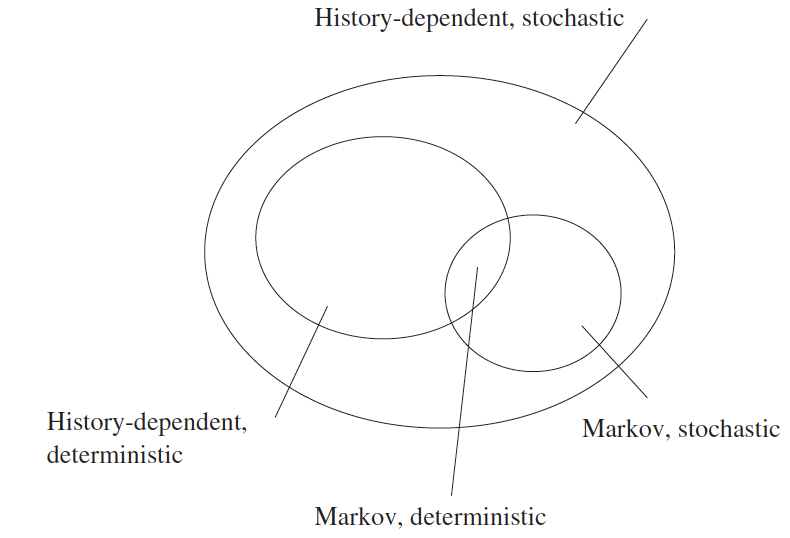
\includegraphics[width= 7cm, height = 6.5cm]{Policies_schema.png}
	\caption{Relationship between different sets of policies~\cite{Sigaud:2010:MDP:1841781}.}
	\label{fig:Policies_schema}
\end{figure}

As shown in figure \ref{fig:Policy_application_schema} each time an agent performs an action $a\textsubscript{t}$ in a state $s\textsubscript{t}$, it receives a real-valued reward $r\textsubscript{t}$ that indicates the immediate value of this state-action transition. This produces a sequence of states $s\textsubscript{i}$, actions $a\textsubscript{i}$, and immediate rewards $r\textsubscript{i}$ as shown in the figure. The agent's task is to learn a control policy, $\{\pi : S \longrightarrow A\}$, that maximizes the expected sum of these rewards, with future rewards discounted exponentially by their delay~\cite{Mitchell}.

\begin{figure}[h!]
	\centering
	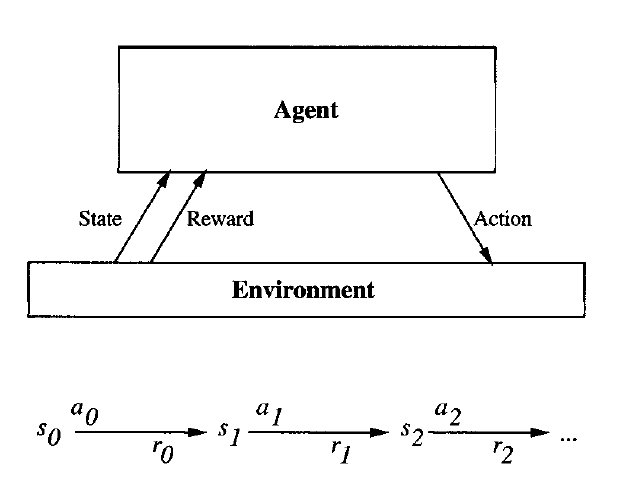
\includegraphics[width= 12cm, height = 10cm]{RLSchema.png}
	\caption{Policy application schema~\cite{SuttonBarto}.}
	\label{fig:Policy_application_schema}
\end{figure}
 
As previously said, the final goal of an optimal policy is to gather the greatest reward possible. In MDPs, there are several ways of taking into account the future in the current behaviour but there are basically three models of optimality which are sufficient to cover most of the approaches in the literature :

\begin{figure}[h!]
\begin{equation*}
E[\sum_{t = 0}^h r_t]
\qquad
E[\sum_{t = 0}^\infty \gamma^t r_t]
\qquad
\lim\limits_{h \rightarrow \infty} E[\dfrac{1}{h} \sum_{t = 0}^h r_t]
\end{equation*}
\caption{Optimality : \textbf{a)} finite horizon, \textbf{b)} discounted, infinite horizon, \textbf{c)} average reward}
\end{figure}

Note that $E[\cdot]$ denotes the expectation operator.

\paragraph{Discount Factor}The \textit{finite horizon} model simply takes a finite horizon of length $h$ and states that the agent should optimize its expected reward over this horizon. In the \textit{infinite-horizon model}, the long-run reward is taken into account, but the rewards that are received in the future are discounted according to how far away in time they will be received.
A \textit{discount factor} $\gamma$, with $0 \leq \gamma \leq 1$ is used for this. Note that in the discounted case, rewards obtained later are discounted more than rewards obtained earlier. Additionally, the discount factor, ensures that, even with infinite horizon, the sum of the rewards obtained is finite. In episodic tasks, i.e. in tasks where the horizon is finite, the discount factor is not
strictly necessary or can equivalently be set to $1$. If $\gamma = 0$ the agent is said to be myopic, which means that it is only concerned about immediate rewards.
The last optimality model is the \textit{average-reward} model. It is useful in maximizing the long-run \textit{average-reward}. Sometimes it is called the \textit{gain optimal} policy and in the limit, it is equal to the infinite-horizon discounted model~\cite{wiering2012reinforcement}

\subsection {Bellman Equation} The concept of \textit{value function} is the link between optimality criteria and policies. Most learning algorithms for MDPs compute optimal policies by learning value functions. The value of a state $s$ under policy $\pi$, denoted $V^\pi (s)$ is the expected return when starting in $s$ and following $\pi$ thereafter. Using the infinite-horizon, discounted model :

\begin{equation}
	V^\pi (s) = E_\pi \{\sum_{k = 0}^{\infty} \gamma^k r\textsubscript{t+k} | s_t = s\}
\end{equation}

A similar state-action value function : $Q : S$ x $A \rightarrow \mathbb{R}$ can be defined as the expected return starting from state $s$, taking action $a$ and thereafter following policy $\pi$ :

\begin{equation} \label{eq:2.2}
	Q^\pi (s,a) = E_\pi\{\sum_{k = 0}^{\infty} \gamma^k r\textsubscript{t+k} | s_t = s, a_t = a\}
\end{equation}

For any policy $\pi$ and any state $s$ the expression \ref{eq:2.2} can recursively be defined in terms of a so-called \textit{Bellman Equation} :

\begin{equation}
\begin{split}
	V^\pi (s) = E_\pi\{r_t + \gamma\textsubscript{t+1} + \gamma^2 r\textsubscript{t+2} + ... | s_t = s\} \\
	= E_\pi \{r_t + \gamma V^\pi(s\textsubscript{t+1}) | s_t = s\} \\
	\sum_{s'}p(s, \pi(s), s') (R(s, a, s') + \gamma V^\pi (s'))
\end{split}	
\end{equation}

It denotes that the expected value of state is defined in terms of immediate reward and values of possible next state weighted by the transition probabilities, and additionally a discount factor. Note that multiple policies can have the same value function, but for a given policy $\pi$, $V^\pi$ is unique. The goal for any MDP is to find a best policy, i.e. a policy that receives the most reward. This means maximizing the value function of equation \ref{eq:2.2} for all states $s \in S$. An optimal policy, denoted $\pi^*$, is such that $V\textsuperscript{$\pi$*} (s) \geq V^\pi (s)$ for all $s \in S$ and all policies $\pi$ :

\begin{equation} 
\label{eq:2.5}
V^*(s) = \max_{a \in A} \sum_{s'}p(s, \pi(s), s') (R(s, a, s') + \gamma V^\pi (s'))
\end{equation}

This expression is called the \textit{Bellman optimality equation}. It states that the value of a state under an optimal policy must be equal to the expected return for the best action in a state~\cite{wiering2012reinforcement}.

\subsection{Value Iteration vs Policy Iteration} Before studying how to solve MDPs, let's clarify the main differences between two key concepts that will be recursively find : \textit{value iteration} and \textit{policy iteration}. \\

Both value iteration and policy iteration, compute the same thing (all optimal values), i.e. they work with Bellman updates. In value iteration one starts with a random value function and then he finds a new (improved) value function in an iterative process, until reaching the optimal value function. Value iteration computation of Bellman Equation is:

\begin{equation}
	V\textsubscript{k+1}(s) \leftarrow \max_{a} \sum_{s'} p(s, a, s') [R(s, a, s') + \gamma V_k(s')]
\end{equation}

\begin{figure}[h!]
	\centering
	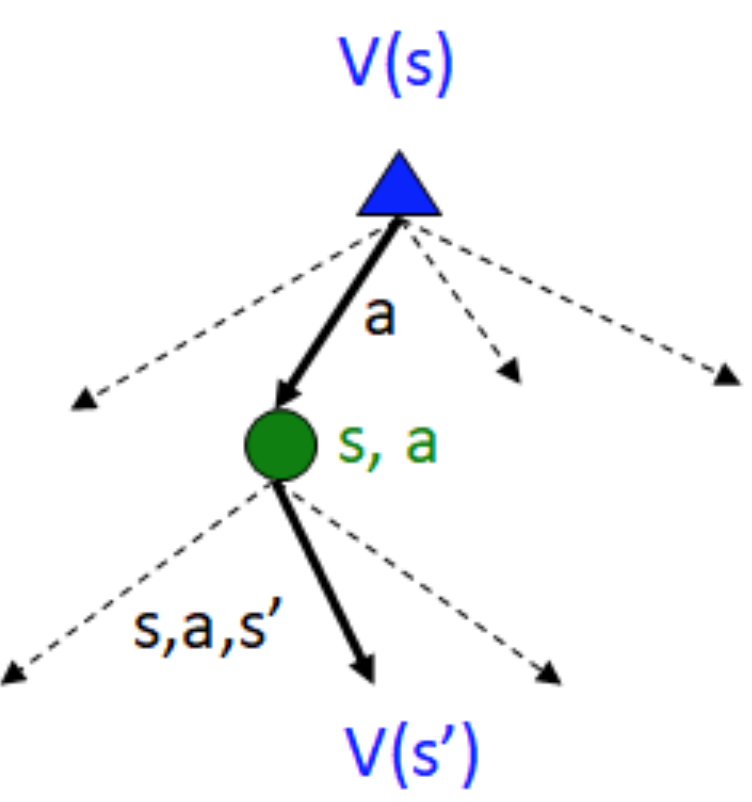
\includegraphics[width= 5cm, height = 5cm]{ValueIterationPolicy.png}
	\caption{Value Iteration Schema}
	\label{fig:ValueiterationPolicy}
\end{figure}

Value iteration has three disadvantages: it is slow ($O(S^2A)$ per iteration), the $\max$ at each state rarely changes, the policy often converges long before the values (figure \ref{fig:ValueiterationPolicy}). \\

Policy iteration computations of Bellman Equation can be classified as :

\begin{itemize}
	\item Evaluation : for a fixed current policy $p$, find values with policy evaluation:
		\begin{equation}
			V\textsupsub{$\pi_i$}{$k+1$}(s) \leftarrow \sum_{s'}p(s, \pi_i(s), s')[R(s, \pi_i(s), s') + \gamma V\textsupsub{$\pi_i$}{k}(s')]
		\end{equation}
	
	\item Improvement : for fixed values, get a better policy using policy extraction :
	
	\begin{equation}
		\pi\textsubscript{i+1}(s) = \arg \max_{a} \sum_{s'} p(s, a, s')[R(s, a, s') + \gamma V\textsuperscript{$\pi_i$}(s')]
	\end{equation}
\end{itemize}

\begin{figure}[h!]
	\centering
	\includegraphics[width= 5cm, height = 5cm]{Policyiteration.png}
	\caption{Policy Iteration Schema}
	\label{fig:PolicyIteration}
\end{figure}

The complexity of policy iteration is $O(S^2)$. \\

Summarizing what said until now, it is possible to write that in policy iteration : \\ 

\begin{itemize}
	\item Every iteration updates both the values and, implicitly, the policy;
	\item The policy is not tracked, but tacking the $\max$ over actions, it is implicitly possible to recompute it.
\end{itemize}

In policy iteration :

\begin{itemize}
	\item Several passes that update utilities with fixed policy are made;
	\item After the policy is evaluated, a new policy is chosen;
	\item The new policy will be always better until the end.
\end{itemize}

\section{Solving MDP}
Now that the main concepts related to MDP, policy, optimality criteria and value function, have been formally defined, it is time to consider the question of how to solve an MDP computing an optimal policy $\pi^*$. Several dimensions exists along which algorithms have been developed for this purpose. The most important distinction is that between \textit{model-based} and \textit{model-free} algorithms ~\cite{wiering2012reinforcement}.

\begin{table}[h!]
	\resizebox{\textwidth}{!}{ 
		\begin{tabular}{|c|| c|c|}
			\hline 
			&\textbf{Model-based algorithms}  &\textbf{Model-free algorithms}  \\ 
			\hline
			\hline \textbf{General name} 
			&DP  &RL  \\ 
			\hline \textbf{Basic assumption} 
			&\thead{A model of the MDP is known \\ beforehand, and can be used to compute \\ value functions and policies using \\ the Bellman equation.}  &\thead{Rely on interaction with the environment. \\ Because a model of the MDP\\ is not known, the agent has\\ to explore the MDP to obtain information.}  \\
			\hline \textbf{Planning} 
			&Yes  &Yes  \\ 
			\hline \textbf{Learning} 
			&No  &Yes  \\ 
			\hline 
		\end{tabular} 
	}
	\caption{Main differences between model-based and model-free algorithms.}
\end{table}

\subsection{Dynamic Programming} The term Dynamic Programming (DP) refers to a class of algorithms that is able to compute optimal policies when a perfect model of the environment described as a Markov Decision Process, exists. Those algorithms are known as \textit{planning algorithms}. In planning algorithms, the idea is that some description of a starting state or states, a goal state or states, and some set of possible actions that the agent can take, are given. The objective is to search through a tree that is the sequences of actions that can be taken, and try to find a nice short plan. In so doing two of the possible planning algorithms are {\tt BFS algorithm} and {\tt DFS algorithm}. \\

The method of Dynamic Programming systematically records solutions for all sub-problems of increasing lengths. Using this programming paradigm the optimal policy is constructed through the step-by-step definition of optimal sub-policies. According to Bellman optimality principle, \textit{all optimal sub-policies of an optimal policy are optimal sub-policies}. DP algorithms are obtained by turning Bellman equations into update rules for improving approximations of the desired value functions.

Studying DP it is possible to distinguish between two different main methods. \textit{Policy evaluation} refers to the typically iterative computation of the value functions for a given policy. \textit{Policy improvement} refers to the computation of an improved policy given the value function for that policy. Either of these can be used to reliably compute optimal policies and value functions for finite MDPs given complete knowledge of the MDP itself.


Classical DP methods operate in sweeps through the state set, performing an \textit{expected update} operation on each state. Each such operation updates the value of one state based on the values of all possible successor states and their probabilities of occurring. Expected updates are closely related to Bellman equations: they are little more than these equations turned into assignment statements. When the updates no longer result in any changes in value, convergence has occurred to values that satisfy the corresponding Bellman Equation~\cite{SuttonBarto}. \\

The assumption that a model is available will be hard to ensure for many applications, however DP algorithms are very relevant because they define fundamental computational mechanisms which can be also used when no model is available. 

\subsection{Reinforcement Learning}
Dynamic Programming' s methods compute optimal policies for an MDP assuming that a perfect model is available. Reinforcement Learning (or \textit{approximate dynamic programming}, or \textit{neuro-dynamic programming}) is primarily concerned with how to obtain an optimal policy when such a model is not available. RL adds to MDPs a focus on approximate and incomplete information, and the need for sampling and exploration. In contrast with DP's algorithms, model-free methods do not rely on the availability of priori known transition and reward models. The lack of the model generates a need to \textit{sample} the MDP to gather statistical knowledge about this unknown model. Many model-free RL techniques exist that probe the environment by doing actions, thereby estimating the same kind of state value and state-action value functions as model-based techniques~\cite{wiering2012reinforcement}.\\

Roughly speaking Reinforcement Learning (RL) is the problem faced by a learner that must behaviour through trial-and-error interactions with a dynamic environment. It can be considered a problem of mapping situations to actions in order to maximize a numerical reward signal~\cite{RLDef1}. \\

In RL the learner must select an action to take at each time step: every choice done by the agent changes the environment in an unknown fashion and receives a reward which value is based on the consequences. The objective of the learner is to choose a sequence of actions based on observations of the current environment that maximizes cumulative reward or minimizes cumulative cost over all time steps~\cite{LiMalik}. The general class of algorithms that interact with the environment and update their estimates after each experience is called \textit{online} RL.

\begin{algorithm}
	\ForEach{episode}{
		$s \in S$ is initialized as the starting state\;
		$t := 0$\;
		\Repeat{$s'$ is a goal state}{
			choose an action $a \in A(s)$\;
			perform action $a$ \;
			observe the new state $s'$ and, received reward $r$, update $\tilde{T}, \tilde{R}, \tilde{Q}$ and/or $\tilde{V}$ using the experience $\bigl \langle$$s, a, r, s'$$\bigr\rangle$\;
			$s:=s'$\;
		}
		
	}
	\caption{A general algorithm for online RL~\cite{wiering2012reinforcement}}
\end{algorithm}

Studying RL, one of the main aspect is the distinction between \textit{direct} and \textit{indirect} Reinforcement Learning. The difference between these two approaches is shown in table \ref{tab:RL_possibilities_schema}. \\

\begin{table}[h!]
	\resizebox{\textwidth}{!}{ 
		\begin{tabular}{|c|| c|c|}
			\hline 
			&\textbf{Model-based/Indirect}  &\textbf{Model-free/Direct}  \\ 
			\hline
			\hline \textbf{Basic Assumption} 
			& \thead{First of all it is necessary \\ to learn the transition and \\ reward model from interaction \\ with the environment. After that, when \\ the model is (approximately or sufficiently) \\ correct, all the DP methods previously described \\ can be applied. } & \thead{It is possible to estimate \\ values of functions, without even \\ estimating the model of the MDP.}  \\ 
			\hline 
		\end{tabular} 
	}
	\caption{RL's approaches classification.}
	\label{tab:RL_possibilities_schema}
\end{table}

RL is different both from \textit{supervised learning} and from \textit{unsupervised learning}. It is not a sample of learning from a training set of labelled examples provided by a knowledgeable external supervisor (\textit{supervised learning}) and it is not a sample of searching and finding structure hidden in a collection of unlabelled data (\textit{unsupervised learning}). More specifically RL can be distinguished from other forms of learning based on the following characteristics :

\begin{itemize}
	\item Reinforcement Learning deals with temporal sequences. In contrast with non-supervised learning problems where the order in which the examples are presented is not relevant, the choice of an action at a given time step will have consequences on the examples that are received at a subsequent time steps~\cite{Sigaud:2010:MDP:1841781}.
	\item In contrast with supervised learning, the environment does not tell the agent what would be the best possible action. Instead, the agent may just receive a scalar reward representing the value of its action and it must \textit{explore} the possible alternative actions to determine whether its action was the best or not~\cite{Sigaud:2010:MDP:1841781}.
\end{itemize}

According to what just said, one of the challenges that arises in RL, and not in other kind of learning, is the trade-off between \textit{exploration} and \textit{exploitation}. To obtain an higher reward, an RL agent must prefer actions that it has tried in the past and found to be effective in producing reward. In order to discover such actions, it has to try actions that it has not selected before. The agent \textit{exploits} what it has already experienced in order to obtain reward, but it has also to \textit{explore} in order to eventually make better action selections in the future~\cite{SuttonBarto}. In other words \textit{exploitation} consists of doing again actions which have proven fruitful in the past, whereas \textit{exploration} consists of trying new actions, looking for a larger cumulated reward, but eventually leading to a worse performance. Dealing with the exploration/exploitation trade-off, consists of determining how the agent should explore to get as fast as possible a policy that is optimal or close enough to the optimum. The most basic exploration strategy is the $\epsilon$-greedy policy, i.e. the learner takes its current best action with probability $(1-\epsilon)$ and a (randomly selected) other action with probability $\epsilon$. ~\cite{Sigaud:2010:MDP:1841781}. 

\subsection{Monte Carlo Methods} Monte Carlo Methods (MC)  represent a first instance of model-free RL's algorithms. They are one way to solve the Reinforcement Learning problem based on averaging sample returns.

The Monte Carlo approach consists of performing a large number of trajectories from all states $s$ in $S$, and estimating $V(s)$ as an average of the cumulated rewards observed along these trajectories. In each trial, the agent records its transitions and rewards, and updates the estimations of the value of the  encountered states according to a discounted reward scheme. The value of each state then converges to $V^\pi (s)$ for each $s$ if the agent follows policy $\pi$.

More formally, let $(s_0, s_1, ..., s_N)$ be a trajectory consistent with the policy $\pi$ and the unknown transition function $p()$, and let $(r_1, ..., r_N)$ be the rewards observed along this trajectory. In MC method, the $N$ values $V(s_t), \quad t = 0, ...., N-1$ are updated according to :

\begin{equation} 
\label{eq:2.6}
V(s_t) \leftarrow V(s_t) + \alpha(s_t)(r\textsubscript{t+1} + r\textsubscript{t+2} + ... + r_N - V(s_t))
\end{equation}

with the learning rates $\alpha(s_t)$ converging to $0$ along the iterations~\cite{Sigaud:2010:MDP:1841781} . MC algorithms treat the long-term reward as a random variable and use its to estimate the sampled mean. Because the sampling is dependent on the current policy $\pi$, only returns for actions suggested by $\pi$ are evaluated. Thus, \textit{exploration} is of key importance here, just as in other model-free methods. One way of ensuring enough exploration is to use exploring starts, i.e. each state-action pair has a non-zero probability of being selected as the initial pair.

A distinction can be made between \textit{every-visit} MC, which averages over all visits of a state $s \in S$ in all episodes, and \textit{first-visit} MC, which averages over just the returns obtained from the first visit to a state $s \in S$ for all episodes. Both variants will
converge to $V^\pi$ for the current policy $\pi$ over time~\cite{wiering2012reinforcement} .

Studying RL methods it is necessary to distinguish between \textit{on-policy methods} and \textit{off-policy methods}.
On-policy methods attempt to evaluate or improve the policy that is used to make decisions. Off-policy methods evaluate or improve a policy different from that used to generate the data. MC methods can be used for both on-policy and off-policy control, and the general pattern complies with the generalized policy iteration procedure. 

\begin{table}
\centering
\begin{tabular}{|c|c|c|}
	\hline 
	&\textbf{On-policy methods}  &\textbf{Off-policy methods}  \\ 
	\hline \textbf{Basic assumption}
	& \thead{They attempt to evaluate\\ or improve the policy that\\ is used to make decisions.}  &\thead{No specific policy \\ is required to be followed; \\ the agent could \\ even behave randomly and \\ despite this it can still  \\ find the optimal policy. }  \\ 
	\hline 
\end{tabular}
\caption{Difference between on-policy and off-policy methods.}
\end{table} 

\subsection{Temporal Difference Learning} An important problem faced by RL is the so called \textit{temporal credit assignment problem}. In model-free contexts it is difficult to assess the utility of some action, if the real effects of this particular action can only be perceived much later. One possibility is to wait until the ”end” (e.g. of an episode) and punish or reward specific actions along the path taken. However, this will take a lot of memory and often, with ongoing tasks, it is not known beforehand whether, or when, there will be an ”end”. Instead, one can use similar mechanisms as in value iteration to adjust the estimated value of a state based on the immediate reward and the estimated (discounted) value of the next state. This is generally called \textit{temporal difference learning} and it is a general mechanism underlying the model-free methods~\cite{wiering2012reinforcement}. \\ 

The basic temporal difference algorithm is $TD(0)$. This algorithm relies on a comparison between the actually received reward and the reward expected from the previous estimations.

If the estimated values $V(s_t)$ and $V(s\textsubscript{t+1})$ in states $s_t$ and $s\textsubscript{t+1}$ were exact, one would have 

\begin{equation}
	V(s_t) = r\textsubscript{t+1} + \gamma r\textsubscript{t+2} + \gamma^2 r\textsubscript{t+3} + ...,
\end{equation}

\begin{equation}
	V(s\textsubscript{t+1}) = r\textsubscript{t+2} + \gamma r\textsubscript{t+3} + \gamma^2r\textsubscript{t+4} + ... .
\end{equation}

Thus one would have 

\begin{equation}
	V(s_t) = r\textsubscript{t+1} + \gamma V(s\textsubscript{t+1}).
\end{equation}

The temporal difference error

\begin{equation}
	\delta_t = r\textsubscript{t+1} + \gamma V(s\textsubscript{t+1}) - V(s_t)
\end{equation}

measures the error between the current estimation $V(s_t)$ and the corrected estimation $r\textsubscript{t+1} + V(s\textsubscript{t+1})$. The temporal difference method consists of correcting this error little by little by modifying $V()$ according to a Windrow-Hoff equation :

\begin{equation}
	V(s_t) \leftarrow V(s_t) + \alpha[r\textsubscript{t+1} + \gamma V(s\textsubscript{t+1}) - V(s_t)] = V(s_t) + \alpha \delta_t .
\end{equation}

Like Monte Carlo methods, TD ones perform estimation of action-value functions based on the experience of the agent and can do it without a model of the underlying MDP; however, they combine this estimation using local estimation propagation mechanisms coming from dynamic programming, resulting in their incremental properties. Thus TD methods, which are at the heart of most reinforcement learning algorithms, are characterized by this combination of estimation methods with local updates incremental properties~\cite{Sigaud:2010:MDP:1841781}.

\subsection{Sarsa Algorithm : On-policy TD Control} Knowing the exact value of all states is not always enough to determine how to proceed. If the agent does not know which action results in reaching any particular state, i.e. if the agent does not have a model of the transition function, knowing $V$ does not help it determine its policy.  To solve this problem, Watkins ~\cite{watkins1992q} introduced the action-value function $Q$, whose knowledge is similar to the knowledge of $V$ when $p$ is known. The action-value function of a fixed policy $\pi$ whose value function is $V^\pi$ is :

\begin{equation}
	\forall s \in S, a \in A, \quad Q^\pi (s,a) = R(s, a) + \gamma \sum_{s'} p(s' \ s, a) V^\pi (s').
\end{equation}

The value of $Q^\pi(s,a)$ is interpreted as the expected value starting from $s$, executing $a$ and then following the policy $\pi$. Having $V^\pi(s) = Q^\pi(x, \pi(x))$, the corresponding Bellman equation is :

\begin{equation}
	\forall s \in S, a \in A \quad Q^*(s, a) = R(s, a) + \gamma \sum_{s'}p(s' | s, a) \max_{b} Q^*(s', b)
\end{equation}

Than :

\begin{equation}
\forall s \in S, \quad V^*(s) = \max_{a} Q^* (s,a ), \quad \pi^*(s) = \arg\max_{a} Q^*(s,a).
\end{equation}

The SARSA algorithm works on state-action pairs rather than on states. Its update equation is :

\begin{equation}
\label{eq:2.12}
Q(s_t, a_t) \leftarrow Q(s_t, a_t) + \alpha[r\textsubscript{t+1} + \gamma Q(s\textsubscript{t+1}, a\textsubscript{t+1}) - Q(s_t, a_t)].
\end{equation}

the information necessary to perform such an update is $(s_t, a_t, r\textsubscript{t+1}, s\textsubscript{t+1}, a\textsubscript{t+1})$, hence the name of the algorithm : SARSA. This algorithm suffers from one conceptual drawback: performing the updates as stated above implies knowing in advance what will be the next action $a\textsubscript{t+1}$ for any possible next state $s\textsubscript{t+1}$.  As a result, the learning process is tightly coupled to the current policy (the algorithm is called "on-policy") and this complicates the exploration process. As a result, proving the convergence of SARSA was more difficult than proving the convergence of "off-policy" algorithms such as Q-learning. Empirical studies often demonstrates the better performance of SARSA compared to Q-learning~\cite{Sigaud:2010:MDP:1841781}.

\begin{algorithm}
	Initialize $Q(s, a)$ arbitrarily\;
	Repeat the next cycle until $s$ is terminal\;
	\ForEach{epsiode}{
	Initalize $s$\;
	Choose $a$ from $s$ using policy derived from $Q$ (e.g. $\epsilon$-greedy)\;
	\ForEach{step of episode}{
		Take action $a$, observer $r$, $s'$\;
		Choose $a'$ from $s'$ using policy derived from $Q$ (e.g. $\epsilon$-greedy)\;
		$Q(s,a) \leftarrow Q(s,a) + \alpha[r + \gamma Q(s', a') - Q(s, a)]$ \;
		$s \leftarrow s'$ \;
		$a \leftarrow a'$ \;
	}
} 
\caption{SARSA Algorithm : On-policy TD Control}
\end{algorithm}

\subsection{Q-learning Algorithm : Off-policy TD Control} The Q-Learning Algorithm can be seen as a simplification of the SARSA algorithm, given that it is no more necessary to determine the action at the next step to calculate updates. Its update equation is :

\begin{equation}
\label{eq:2.13}
	Q(s_t, a_t) \leftarrow Q(s_t, a_t) + \alpha[r\textsubscript{t+1} + \gamma \max_{a} Q(s\textsubscript{t+1}, a) - Q(s_t, a_t)]
\end{equation} 

\begin{algorithm}
	$\alpha_t$ is the learning rate \;
	Initialize ($Q_0$)\;
	\For{$t = 0$ ; $t \leq T\textsubscript{tot} - 1$ ; $t++$}{
		$s_t \leftarrow {\tt ChooseState}$\;
		$a_t \leftarrow {\tt ChooseAction}$\;
		$s\textsubscript{t+1}, r\textsubscript{t+1} \leftarrow {\tt Simulate}(s_t, a_t)$\;
		update $Q_t$ \;
		\Begin{
			$Q\textsubscript{t+1} \leftarrow Q_t$\;
			$\delta_t \leftarrow r\textsubscript{t+1} + \gamma \max_{b} Q_t (s\textsubscript{t+1}, b) - Q_t(s_t, a_t)$ \;
			$Q\textsubscript{t+1}(s_t, a_t) \leftarrow Q_t(s_t, a_t) + \alpha_t(s_t, a_t) \delta_t$ \;
		}
	}
\KwRet{Q\textsubscript{Tot}}
\caption{Q-learning Algorithm ~\cite{Sigaud:2010:MDP:1841781}}
\end{algorithm}

The main difference between SARSA and Q-Learning lies in the definition of the error term. The $Q(s\textsubscript{t+1}, a\textsubscript{t+1})$ term in the equation \ref{eq:2.12}	is replaced by $\max_{a}Q(s\textsubscript{t+1}, a)$ in equation \ref{eq:2.13}. Updates are based on instantaneously available information. In this algorithm, the $T\textsubscript{tot}$ parameter corresponds to the number of iterations. There is here one learning rate $\alpha_t(s, a)$ for each state-action pair, it decreases at each visit of the corresponding  pair. The {\tt Simulate} function returns a new state and the corresponding reward according to the dynamics of the system. The choice of the current state and of the executed action is performed by functions {\tt ChooseState} and {\tt ChooseAction}. The {\tt Initialize} function initializes the $Q$ function with $Q_0$, which is often initialized with {\tt null} values, whereas more adequate choices can highly improve the performance~\cite{Sigaud:2010:MDP:1841781}.

\subsection{SARSA($\lambda$) Algorithm} Previously described algorithms only perform one update per time step in the state the agent is visiting. This update process is particularly slow. Indeed, an agent deprived of any information on the structure of the value function needs at least $n$ trials to propagate the immediate reward of a state to another state that is $n$ transitions away. Before this propagation is achieved, if the initial values are {\tt null}, the agent performs a random walk in the state space, which means that it needs an exponential number of steps as a function of $n$ before reaching the reward "trail" (figure \ref{fig:NonLambda}).

\begin{figure}[h!]
	\centering
	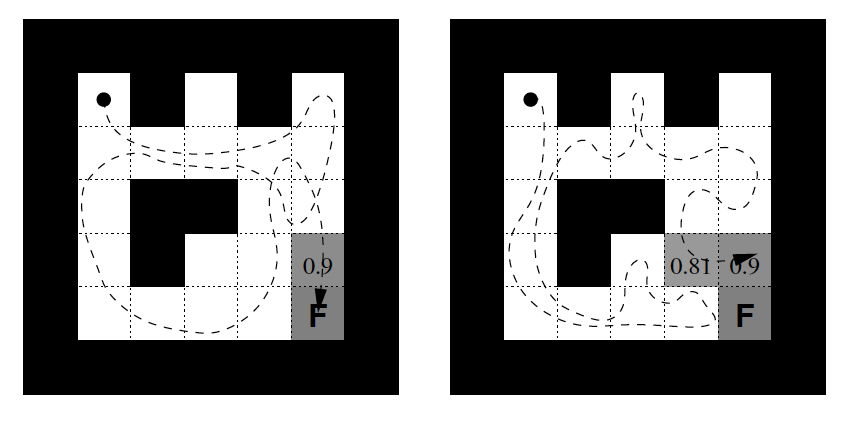
\includegraphics[width= 10cm, height = 5cm]{NonLambda}
	\caption{Q-learning : first and second trial. It can be seen that, all values being initially {\tt null}, the propagation of {\tt non-null} values does not starts until the agent finds the reward source for the first time, and only progress once per trial~\cite{Sigaud:2010:MDP:1841781}.}
	\label{fig:NonLambda}
\end{figure}

A naive way to solve the problem consists of using a memory of trajectory and to propagate all the information backwards along the performed transitions each time a reward is reached. Such a memory of performed transitions is called an ''eligibility trace''. A problem with this naive approach is that the required memory grows with length of trajectories, which is obviously not feasible in the infinite horizon context. In SARSA($\lambda$) algorithm, a more sophisticated approach that addresses the infinite horizon context is used. \\

As already saw, Q-learning integrates the temporal difference error idea. With the update rule of Q-learning :

\begin{equation}
	Q\textsubscript{t+1} (s_t, a_t) = Q_t(s_t, a_t) + \alpha_t\{r\textsubscript{t+1} + \gamma V_t(s\textsubscript{t+1}) - Q_t(s_t, a_t)\}
\end{equation}

for transition ($s_t, a_t, s\textsubscript{t+1}, r\textsubscript{t+1}$), and in the case where action $a_t$ executed in state $s_t$ is the optima action for $Q_t$, then the error term is $r\textsubscript{t+1} + \gamma V_t s\textsubscript{t+1} - V_t(s_t)$. For a generic parameter $\lambda \in [0,1]$ it can be generalized as shown in algorithm \ref{SarsaLambdaAlgo}.

\begin{algorithm}
	/* $\alpha$ is a learning rate */ \;
	{\tt Initialize} $Q_0$ \;
	$z_0 \leftarrow 0$ \;
	$s_0 \leftarrow$ {\tt ChooseState} \;
	$a_0 \leftarrow$ {\tt ChooseAction} \;
	$t \leftarrow 0$ \;
	\While{$t \leq  T\textsubscript{tot}-1$}{
		($s_t', r\textsubscript{t+1}$) $\leftarrow$ {\tt Simulate} $(s_t, a_t)$ \;
		$a_t' \leftarrow$ {\tt ChooseAction} \;
		update $Q_t$ and $z_t$ \;
		\Begin{
			$\delta_t \leftarrow r\textsubscript{t+1} + \gamma Q_t(s_t', a_t') - Q_t(s_t, a_t)$ \;
			$z_t(s_t, a_t) \leftarrow z_t(s_t, a_t) + 1$ \;
			\For{$s \in S, a \in A$}{
				$Q\textsubscript{t+1}(s, a) \leftarrow Q_t(s, a) + \alpha_t(s,a)z_t(s,a)\delta_t$ \;
				$z\textsubscript{t+1}(s,a) \leftarrow \gamma\lambda z_t(s,a)$
			}
		\If{$s_t'$ non absorbing}{
				$s\textsubscript{t+1} \leftarrow s_t'$ and $a\textsubscript{t+1} \leftarrow a_t'$ \;
			}
		\Else{
				$s\textsubscript{t+1} \leftarrow$ {\tt ChooseState} \;
				$a\textsubscript{t+1} \leftarrow$ {\tt ChooseAction} \;
			}
		}
	}
\KwRet{$Q\textsubscript{Tot}$}
\caption{SARSA ($\lambda$) Algorithm \cite{Sigaud:2010:MDP:1841781}}
\label{SarsaLambdaAlgo} 
\end{algorithm}

Here $z_t(s, a)$  is the eligibility trace and \textit{absorbing state} is the terminal state~\cite{Sigaud:2010:MDP:1841781}. The eligibility trace represents a short-term memory vector, \textbf{z\textsubscript{t}} $\in \mathbb{R}^d$, that parallels the long-term weight vector \textbf{w\textsubscript{t}} $\in \mathbb{R}^d$. The rough idea is that when a component of \textbf{w\textsubscript{t}} participates in producing an estimated value, then the  corresponding component of \textbf{z\textsubscript{t}} is bumped up and then begins to fade away. Learning will then occur in that component of \textbf{w\textsubscript{t}} if a non-zero TD error occurs before the trace falls back to zero. The trace-decay parameter $\lambda \in [0, 1]$ determines the rates at which the trace falls \cite{SuttonBarto}. In other words, an eligibility trace is a parameter used to control the “memory” of the algorithm, associated to a given state, enabling the assignment of more credit, e.g. higher trace, to the states and actions performed closer to the end of the episode.

\begin{figure}[h!]
	\centering
	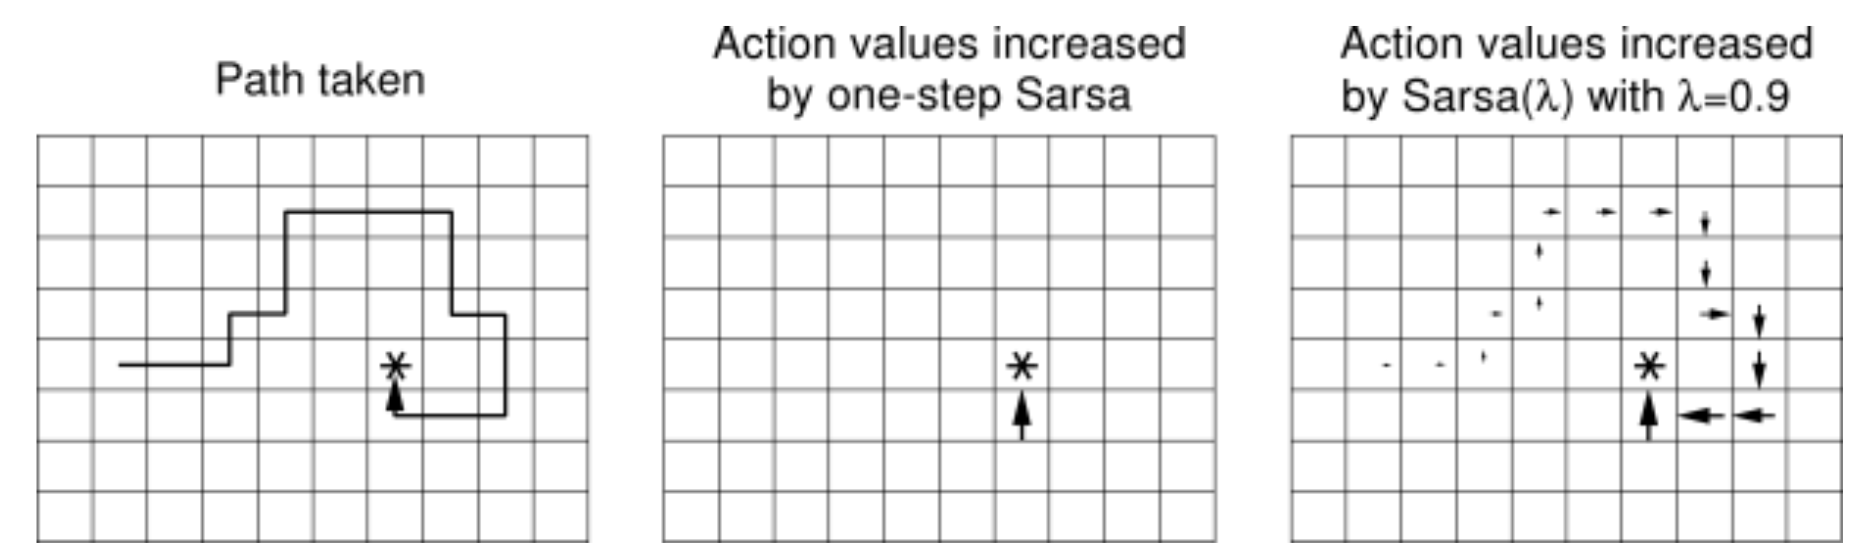
\includegraphics[width= 12cm, height = 5cm]{SarsaLambdaTD}
	\caption{Grid-world example of the speed up of policy learning due to the use of eligibility traces.}
	\label{fig:SarsaLambdaTD}
\end{figure}

The effect of the $\lambda$ value is still poorly understood and tuning optimally its value for a given problem is still an open empirical problem \cite{Sigaud:2010:MDP:1841781}.


